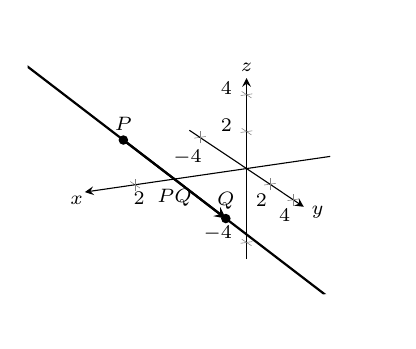
\begin{tikzpicture}[>=stealth]
\begin{axis}%
[width=175pt,tick label style={font=\scriptsize},axis on top,
			axis lines=center,
			view={155}{25},
			name=myplot,
			%xtick={2},
			ytick={-4,2,4},
			ztick={-4,2,4},
			ymin=-4.9,ymax=4.9,
			xmin=-1.5,xmax=2.9,
			zmin=-4.9, zmax=4.9,
			every axis x label/.style={at={(axis cs:\pgfkeysvalueof{/pgfplots/xmax},0,0)},xshift=-3pt,yshift=-3pt},
				xlabel={\scriptsize $x$},
			every axis y label/.style={at={(axis cs:0,\pgfkeysvalueof{/pgfplots/ymax},0)},xshift=5pt,yshift=-2pt},
				ylabel={\scriptsize $y$},
				every axis z label/.style={at={(axis cs:0,0,\pgfkeysvalueof{/pgfplots/zmax})},xshift=0pt,yshift=4pt},
				zlabel={\scriptsize $z$}
			]



\addplot3[domain=-2.5:3.5,thick,samples y=0,{\colorone}] ({2-x},{-1+4*x},{2-3*x});

%\addplot3[domain=-2.5:3.5,thick,samples y=0,{\colorone}] ({2.8-2.9*x},{10.15-4.93*x},{-5.05+6.09*x});

%\draw (axis cs:-1,6,5.8) node [below] {\scriptsize $\ell_2$};



\draw [->,thick,{\colortwo}] (axis cs:2,-1,2) -- (axis cs: 1,3,-1) node [black,below,pos=.5] {\scriptsize $\vv{PQ}$};
%
%\draw (axis cs:2.7,-4,0) node [below] {\scriptsize $\ell_1$};
\filldraw [black] (axis cs:2,-1,2) circle (1.5pt) node [above] {\scriptsize $P$};
\filldraw [black] (axis cs:1,3,-1) circle (1.5pt) node [above] {\scriptsize $Q$};

%\draw [->,thick,black] (axis cs:2.8,10.15,-5.05) -- (axis cs: -.1,5.22,1.04) node [black,right] {\scriptsize $\vec d_2$};
%
%\draw [->,thick,{\colortwo}] (axis cs:0,0,0) -- (axis cs: 1,-1,1) node [black,above] {\scriptsize $\vec p$};
%\draw [->,thick] (axis cs: 0,0,0) -- (axis cs: 0,2,1) node [above,pos=.9] {\scriptsize $\vec p$};
%
%\draw [->,thick] (axis cs: 0,0,0) -- (axis cs: -1,2,2) node [above,pos=.8] {\scriptsize $\vec p+\vec d$};
%
%\draw [->,thick] (axis cs: 0,0,0) -- (axis cs: 2,2,-1) node [left,pos=.9] {\scriptsize $\vec p-2\vec d$};
%
%\draw[>=stealth,->,thick] (axis cs:.1,.1,1.09) -- (axis cs: .7,.1,1.03) node [ left] {\scriptsize $\vec u$};
%
%\filldraw[black] (axis cs: .1,.1,1.09) circle (1pt);
%
%\draw[>=stealth,->,thick] (axis cs:.1,.1,1.09) -- (axis cs: .1,.8,1.79) node [right] {\scriptsize $\vec v$};
%
%\addplot3[domain=0:90,samples y=0,black,thick] ({.3*cos(x)+.1},{.3*sin(x)+.1},{-.1*(.3*cos(x)+.1)+(.3*sin(x)+.1)+1});
%
%\draw (axis cs: .5,.4,1.36) node  {\scriptsize $\theta$};

%\draw (axis cs: 0,0,\pgfkeysvalueof{/pgfplots/zmax}) node [shift={(0,0,20pt)}]{\scriptsize $z$};

%\draw (axis cs: 0,\pgfkeysvalueof{/pgfplots/ymax},0) node [shift={(0,2pt,0)}]{\scriptsize $y$};

%\draw (axis cs: \pgfkeysvalueof{/pgfplots/xmax},0,0) node [shift={(6pt,0,0)}]{\scriptsize $x$};

\end{axis}
%\node [right] at (myplot.right of origin)[shift={(-20pt,-8pt)}] {\scriptsize $y$};
%\node [above] at (myplot.above origin) [shift={(0,-5pt)}] {\scriptsize $z$};
\end{tikzpicture}










